\section{Results and discussion}

In this section we detail the findings of our study. We present the results of the first and
second studies in Section~\ref{sec:res-fs} and Section~\ref{sec:res-ss}. In Section~\ref{sec:discussion} we summarize the
implications of our study. 

\subsection{Result of the first study: A non-exact replication}\label{sec:res-fs}

Our first study is a replication of the \blls.
As discussed in the previous section, to this end, we first executed the analysis using the DroidXP benchmark with its default
configuration. After that, we executed the analysis again, by disabling the DroidFax static analysis algorithm.
In this way, we could better estimate the performance of the dynamic analysis tools for mining Android sandboxes.
Table~\ref{tab:fs} summarizes the results of the executions. The columns Exec. (WS) and Exec. (WOS) 
show the number of malwares identified when executing each tool with the
support of the DroidFax static analysis algorithms (WS) and without the support
of DroidFax static analysis algorithms (WOS). 
The Impact column shows the impact
(in percentage) of DroidFax static analysis algorithms in the results. \kn{Define impact formally, may be as a ratio}

\kn{The following ssentence is kind of stating the obviouss and comes off as an attack already. THis should bee a conclusion box. Did we introduce joke in study? If not please introduce. If yes, please use joke by saying "joke, our ..... improves its performance by"}
Note that, in the \blls, the authors do not present a
discussion about the influence of DroidFax in the results, even
though here we report that the impact of DroidFax in the results is significant, ranging
from 16.44\% (DroidBot) to 51.79\% (Humanoid)---discarding our
\joke tool, the fake tool that does not execute apps during a benchmark execution, for which DroidFax improves its performance by 100\%. This result is
expected, since the \joke tool does not execute any dynamic analysis.
Next we discuss the result of each individual test generation tool. 

\begin{table}[ht]
  \caption{Summary of the results of the first study. }
  \centering
  \begin{small}
 \begin{tabular}{lrrr}
   \toprule
   Tool & Exec. (WS) & Exec. (WOS) & Impact (\%) \\   \midrule
   DroidBot &  73 & 61 & 16.44 \\ 
   Monkey &  71 & 56 & 21.13 \\ 
   DroidMate &  68 & 52 & 23.53 \\ 
   Humanoid &  56 & 27 & 51.79 \\ 
\joke &  42 & 0 & 100.00 \\ 
 \bottomrule
 \end{tabular}
 \end{small}
 \label{tab:fs}
\end{table}

\begin{description}
\item[DroidBot] in the first execution (Exec. WS) led to a sandbox that detected a total of $73$ malware among $96$ pairs present in our dataset ($76.04$\%),
  detecting more apps with malicious behavior than any other tool. Similar to the \blls, DroidBot is the test case generation tool
  whose resulting sandbox detected the largest number of malicious apps. Moreover, in our second execution (Exec WOS), removing the DroidFax
  static analysis support reduced the DroidBot performance in 16.44\%, the smaller impact we observed among the tools.

  \item[Monkey] in the first execution (Exec. WS) produced a sandbox that detected $71$ out of the $96$ pairs of Android apps.
    Contrasting, in the original study, the Monkey's sandbox detected $48$ malwares within the 102 pairs ($47.05$\%). This difference
    might be due to the fact that Monkey uses a random strategy for test case generation and here we considered the outcomes
    of three executions---while in the \blls, the authors consider the outcomes of one execution. 
    Considering our second execution (Exec WOS), there is a reduction of $21.13$\% in the Monkey's performance, leading to
    a sandobox that was able to detect $56$ malwares. 

  \item[DroidMate] in the first execution (Exec. WS) led to a sandbox that detected 68 apps with malicious behavior ($70.83$\%).
    In the \blls study, DroidMate also detected $68$ malwares, though considering the $102$ pairs of apps used in the
    original study. In the second execution(WOS),
    without the DroidFax static analysis algorithms, the resulting sandbox's performance drops by $23.53$\%, being able to detect
    52 out of the 96 pairs of Android apps.
    
  \item[Humanoid] showed the worst performance, even though a previous work~\cite{DBLP:conf/kbse/LiY0C19} presented that it leads to
    the highest number of lines coverage in comparison to Monkey, DroidBot, and DroidMate. In the first execution (Exec. WS),
    the resulting Humanoid sandbox identified $56$ malwares in our dataset ($58.33$\%). Humanoid was the most affected in the second
    execution (Exec. WOS), whose resulting sandbox presents a redunction of $51.79$\%  in the number of detected malwares.
    Since the \blls did not explore Humanoid,
    we do not have a baseline for comparison with the previous work.

  \item[\joke] is our fake test case generation tool that help us understand the performance of the DroidFax static analysis algorithm for mining sandboxes. 
  %\kn{joke seems to be defined here but used before}
    We integrated \joke into the DroidXP benchmark as an additional test case generation tool that does not run the Android apps.
    As a result, the analysis using \joke reveals the performance of DroidFax static analysis algorithms alone. For the first execution, with the DroidFax static
    algorithms enabled, even though \joke does not execute the Android apps, its resulting sandbox detected 43.75\% of the malwares. For the second execution,
    that is, disabling the DroidFax static analysis algorithm, the resulting \joke sandbox was not able to detect any malware. This result
    was expected, since \joke does not analyze the Android apps during the benchmark execution.

\end{description}


\begin{finding}
  Integrating the dynamic analysis tools
  with the DroidFax static analysis algorithms
  improves substantially the performance
  of the resulting Android sandboxes for
  detecting malicious behavior. 
\end{finding}
 
The Venn-diagram of Figure~\ref{fig:venn-plot1}
summarizes how the tools can complement each other.
Note in the diagram that $53$ malwares have been detected
by all sandboxes generated in the first execution (with the DroidFax static analysis algorithms),
out of the 78 identified by at least one sandbox. In addition, the DroidBot sandbox did not detect
any malware that had not been detected by the other tools. Differently, the Monkey sandbox detected
three malwares that had not been detected by any other sandbox, the DroidBot sandbox detected two malwares
that had not been detected by any other sandbox, and the Humanoid sandbox detected one malware that had not
been detected by any other sandbox. \kn{Do our results vary from the results of BLL study or the results claimed by the individual papers themselves. We should talk about this. } Contrasting with the \blls,
our results suggest that using DroidBot in combination with Monkey, DroidMate, and Humanoid
does not improve the general performance of an integrated environment for mining
Android sandboxes.

\begin{finding}
  Our results suggest that one might benefit from using  an integrated
  environment that combines Monkey, DroidMate, and Humanoid to
  mine Android sandboxes. Introducing the DroidBot 
  tool does not improve the results.
\end{finding}


\begin{figure}[htb]
  \centering{
  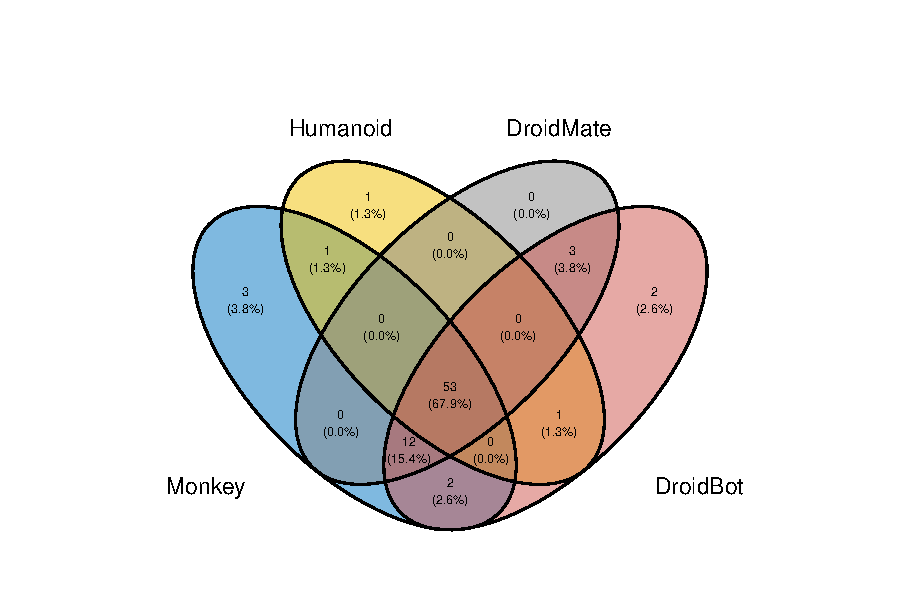
\includegraphics[trim=60 20 0 50,scale=0.7]{images/venn-plot-s1-1.pdf}}
  \caption{Venn Diagram highlighting how the sandboxes from the tools can
    complement each other.}
  \label{fig:venn-plot1}
\end{figure}


Altogether, ignoring the \joke tool, our study reveals that from $58.33$\% (Humanoid)
to $76.04$\% (DroidBot) of the malicious apps investigated in our study can be
detected using the sandboxes generated after running the test case tools with the support of the
DroidFax static analysis algorithms. Besides that, in the first execution, none of the
resulting sandboxes could detect 18 malwares in our dataset ($18.75$\%). According to
the Euphony tool~\cite{hurier2017euphony}, $12$ of these $18$ malwares are \emph{adwares}, $3$ are \emph{trojans}, $2$ are
PUPs (\emph{Potentially Unwanted Program}), and one is an \emph{exploit}.

The DroidBot and Humanoid sandboxes detected the malicious version of the app \texttt{com.andoop.flyracing}. In this particular case, the malicious version changed the Android Manifest file, adding permissions to receive and send SMS messages
(Listing~\ref{lst:androidManifest}). With these permissions, malicious apps may get money fraudulently by sending messages without user confirmation, or may monitor messages or delete them without showing them to user. 
%\kn{Is this the only app where the manifest was changed. If yes, I am not sure we can make broad claims about manifest being a serious place of vulnerabilities.} 
Moreover, after decompiling this malware, we also observed that the malicious version of the
\texttt{MainService} class introduced a
behavior that collects sensitive information (the International Mobile
Equipment Identity, IMEI) and sends it using an SMS message
(Listing~\ref{lst:mainService}). 

\begin{lstlisting}[caption={Diffs in the \texttt{com.gau.screenguru.finger}
      AndroidManifest file of the malicious
      version}, language=Java,
    basicstyle=\fontsize{8}{6}\selectfont\ttfamily,
    label={lst:androidManifest}]

67:M >    <uses-permission android:name="android.permission.RECEIVE_SMS"/>
68:M >    <uses-permission android:name="android.permission.SEND_SMS"/>
\end{lstlisting}

\begin{lstlisting}[caption={Diffs in the malicious version
      of the class \texttt{com.android.main.MainService}
      (app \texttt{com.gau.screenguru.finger})},
      language=Java, basicstyle=\fontsize{8}{6}\selectfont\ttfamily,
      label={lst:mainService}]

492:M > localObject2 = (TelephonyManager)getSystemService("phone");
493:M > if (localObject2 != null)
494:M > {
495:M >  this.imei = ((TelephonyManager)localObject2).getDeviceId();
496:M >  this.imsi = ((TelephonyManager)localObject2).getSubscriberId();
497:M >  this.iccid = ((TelephonyManager)localObject2).getSimSerialNumber();
498:M > }
// [...]
519:M > if ("".equals(this.destMobile)) {
520:M >  getDestMobile();
521:M > }
522:M > sendSMS(this.destMobile, "imei:" + this.imei)
\end{lstlisting}

%% In what follows we present some characteristics of two malwares
%% that had not been detected by the sandboxes (app \texttt{mobi.infolife.cachepro} and app \texttt{com.andoop.flyracing}).

%% In the first example (\texttt{mobi.infolife.cachepro}), the malicious behavior comprises changes to
%% the app idiom (Listing~\ref{lst:app65a}) and to the publisher identifier (Listing~\ref{lst:app65b}).
%% Although such a modification does not threaten the user's device,
%% it might characterize a scenario of app misappropiation.
%% Although such a modification does not threaten the user's device,
%% it might characterize a scenario of app misappropriation. That is, after manually dissecting this particular malware,
%% we did not identify any change with regard to calls to sensitive APIs or app behavior.

%% \begin{lstlisting}[caption= {Diff in the file \texttt{smali/mobi/infolife/cachepro/h.smali}. \texttt{B} stands for
%%     the benign version, while \texttt{M} stands for the malign version.},language=Java, basicstyle=\fontsize{8}{6}\selectfont\ttfamily,label={lst:app65a}]

%% 1:B < const-string v3, "Swith To "
%% ---
%% 1:M > const-string v3, "\u65e0\u6cd5\u542f\u52a8\u5e94\u7528\u201c"
%% \end{lstlisting}

Now we show an interesting case, because none of the computed sandboxes detected the malicious version of the app \texttt{com.andoop.flyracing}. Indeed, the malicious version only changes the Android Manifest file, modifying the meta-data \texttt{ADMOB\_PUBLISHER\_ID}. However, the AdMob is a monetization service provided by Google, and changing the AdMob \emph{publisher identifier} account redirects the advertisement's revenue to another destination. 

\begin{lstlisting}[caption={Diff in the file \texttt{com.andoop.flyracing}
      AndroidManifest file of the malicious version.
      \texttt{B} stands for
      the benign version, while \texttt{M} stands for the malign version.}, language=XML,
    basicstyle=\fontsize{8}{6}\selectfont\ttfamily,label={lst:app65b}]

1:B < <meta-data android:name="ADMOB_\PUBLISHER_\ID"
                     android:value="a14cf7346295891"/>
---
1:M > <meta-data android:name="ADMOB_\PUBLISHER_\ID"
                     android:value="a14f099bfbf3c61"/>
\end{lstlisting}

Differently, the next malicious version app \texttt{com.happymaau.MathRef} was detected by all computed sandboxes. First, the malicious version of package changed the Android Manifest file, adding permissions to access network state and wifi state. These changes allow an app to view the status of all networks and make changes to configured wi-fi networks. (Listing~\ref{lst:androidManifest2}). 


\begin{lstlisting}[caption={Diffs in the \texttt{com.happymaau.MathRef}
      AndroidManifest file of the malicious
      version}.
      , language=XML,
    basicstyle=\fontsize{8}{6}\selectfont\ttfamily,label={lst:androidManifest2}]

165:M >    <uses-permission android:name="android.permission.ACCESS_NETWORK_STATE"/>
166:M >    <uses-permission android:name="android.permission.ACCESS_WIFI_STATE"/>
\end{lstlisting}


We also observed that the malicious version of the \texttt{d} class, introduced a method \texttt{a}, that collects network and wifi information, like Mac address and network state. (Listing~\ref{lst:d})

\begin{lstlisting}[caption={Diffs in the malicious version
      of the class \texttt{com.mn.vymq.b.d}
      (app \texttt{com.happymaau.MathRef})},
      language=Java, basicstyle=\fontsize{8}{6}\selectfont\ttfamily,
      label={lst:d}]

105:M > private String a(Context paramContext)
106:M > {
107:M >	String str = ((TelephonyManager)paramContext.getSystemService("phone")).getDeviceId();
108:M > StringBuilder localStringBuilder = new StringBuilder();
109:M > localStringBuilder.append(str);
110:M > paramContext = (WifiManager)paramContext.getSystemService("wifi");
111:M > if (paramContext == null) {}
112:M >  for (paramContext = null;; paramContext = paramContext.getConnectionInfo())
113:M >  {
114:M >   if (paramContext != null)
115:M >    {
116:M >      paramContext = paramContext.getMacAddress();
117:M >      if (paramContext != null) {
118:M >       localStringBuilder.append(paramContext);
119:M >      }
120:M >    }
121:M >    return a(localStringBuilder.toString());
122:M >  }
123:M > }
\end{lstlisting}

Our last example is a malicious version app \texttt{ru.qixi.android.smartrabbits}. It also was detected by all computed sandboxes, and such as the previous malware example, it changed the Android Manifest file, adding this time, permission to access location sources. This permission allows access location sources, such as the Global Positioning System (GPS) on the phone, where available. Malicious applications can use this resource to determine where the phone user are, and may consume additional battery power. (Listing~\ref{lst:androidManifest3})

\begin{lstlisting}[caption={Diffs in the \texttt{com.happymaau.MathRef}
      AndroidManifest file of the malicious
      version}.
      , language=XML,
    basicstyle=\fontsize{8}{6}\selectfont\ttfamily,label={lst:androidManifest3}]

8:M >    <uses-permission android:name="android.permission.ACCESS_COARSE_LOCATION"/>
9:M >    <uses-permission android:name="android.permission.ACCESS_FINE_LOCATION"/>
\end{lstlisting}

This malicious app clandestinely monitors the geographic location user and sink these information to a web server. The code that follows, show how the method \texttt{c}, from \texttt{q} class, collects these sensitive resource. (Listing~\ref{lst:c}).

\begin{lstlisting}[caption={Diffs in the malicious version
      of the class \texttt{net.crazymedia.iad.d.q}
      (app \texttt{ru.qixi.android.smartrabbits})},
      language=Java, basicstyle=\fontsize{8}{6}\selectfont\ttfamily,
      label={lst:c}]


65:M > private Location c(Context paramContext)
66:M > {
67:M > try
68:M >  {
69:M >  if (Arrays.asList(paramContext.getPackageManager().getPackageInfo
              (paramContext.getPackageName(),4096).requestedPermissions).contains
              ("android.permission.ACCESS_FINE_LOCATION"))

70:M >   {
71:M >    paramContext = (LocationManager)paramContext.getSystemService("location");
72:M >    Criteria localCriteria = new Criteria();
73:M >    localCriteria.setAccuracy(1);
74:M >    localCriteria.setAltitudeRequired(false);
75:M >    localCriteria.setBearingRequired(false);
76:M >    localCriteria.setCostAllowed(true);
77:M >    localCriteria.setPowerRequirement(1);
78:M >    paramContext = paramContext.getLastKnownLocation
                    (paramContext.getBestProvider(localCriteria, true));
                    
79:M >    return paramContext;
80:M >   }
81:M >  }
82:M >  catch (PackageManager.NameNotFoundException paramContext)
83:M >  {
84:M >   paramContext.printStackTrace();
85:M >   return null;
86:M >  }
87:M >  catch (Exception paramContext)
88:M >  {
89:M >   paramContext.printStackTrace();
90:M >  }
91:M >  return null;
92:M > }
\end{lstlisting}


\subsection{Result of the second study: Tainted analysis algorithms.}\label{sec:res-ss}

In this second study we used a tainted analysis approach to mine differences between the benign and malicious versions of each of the 96 Android apps in our dataset. To this end we leverage the FlowDroid
%\kn{ Have we cited flowdroid before. If yes, ignore my comment} 
tool, which tracks how sensitive information flows through the apps using tainted analysis algorithms. Regarding accuracy, the tainted analysis approach detected $58$ out of the $96$ pairs in our dataset ($60,42$\%), that is, the FlowDroid approach leads to a better performance than any sandbox originated in the second execution of the dynamic analysis tools (without the DroidFax static analysis algorithms).


\kn{I see this as a bonus insight. We set out to understand whether static analysis can complement and improve dynamic analysis. But we seem to also have proven that static analysis alone is superior to dynamic analysis. If no other work has touched this topic, we should mention this. I cant recollect any work that compared static analysis tools to dynamic analysis tools. If they have actually done, we should report them}

\begin{finding}
  The performance of FlowDroid to identify malicious behavior
  is superior than the performance of the
  mining sandbox approach supported by dynamic analysis only i.e without
  the DroidFax static analysis algorithms.
\end{finding}

Additionally, we investigate if we could benefit from combining
the results from FlowDroid and DroidFax. Figure~\ref{fig:venn-plot2} shows a
Venn-diagram summarizing the results. So, when combining
the results from FlowDroid and DroidFax, we were able to detect
$67$ of the malicious apps ($69.79$\%), a performance compatible
to that we found as response to the first execution of the
test case generation tools---which also considers the DroidFax
static analysis algorithms. More interesting, from those $67$
malicious apps identified, $33$ pairs had been found by
both tools (FlowDroid and DroidFax), even though they follow
a completely different static analysis approach. Furthermore,
FlowDroid shows to be more effective than DroidFax, detecting $25$ malicious
apps that had not been detected by DroidFax (while DroidFax detected $9$
malicious apps that had not been detected by FlowDroid).

\begin{finding}
  Integrating the results of static analysis tools
  (such as FlowDroid and DroidFax) seems promising,
  leading to a performance similar to that achievend
  when combining test case generation tools with the
  DroidFax tool. 
\end{finding}

\begin{figure}
  \centering{
  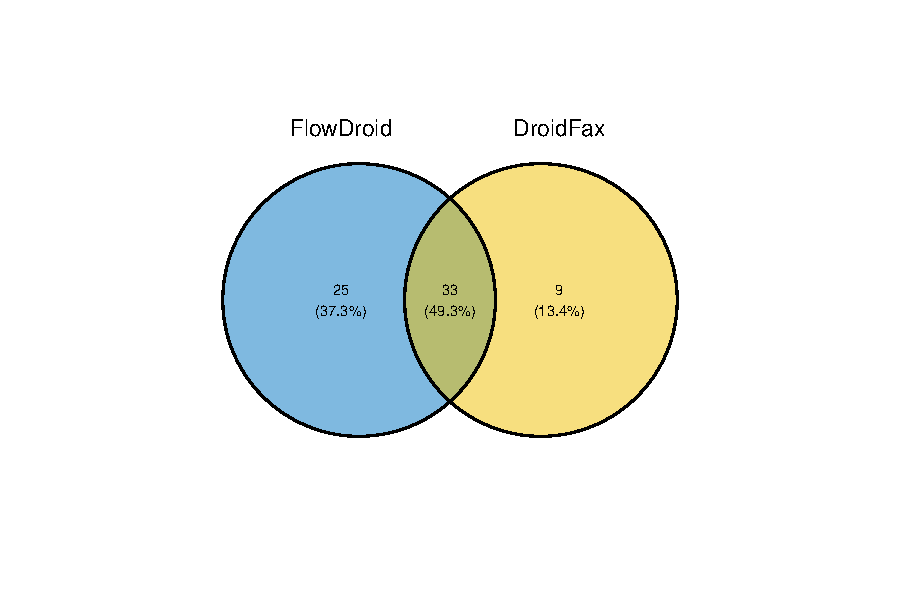
\includegraphics[trim=60 20 0 50,scale=0.7]{images/venn-plot-s2-1.pdf}}
  \caption{Venn Diagram highlighting the possible benefits of
    integrating FlowDroid and DroidFax.}
  \label{fig:venn-plot2}

\end{figure}

The execution of FlowDroid is also feasible: the analysis takes only
32.08 seconds per app on average, totaling a processing time of 52
minutes to analyze all 96 pairs of Android apps.
Even though the time to execute the FlowDroid analysis depends on the size
of the app, the longest run took only 437 seconds. 

Finally, we can highlight that FlowDroid was able to detect $4$ malwares among the $18$ malicious Android apps that had not
been detected by the sandboxes constructed in the first study. Among these
four malwares, $2$ are \emph{trojans}, $1$ is an \emph{exploit}, and 1 is an \emph{adware}.

\begin{finding}
  Although FlowDroid presents a performance similar
  to that of using the dynamic analysis approach for mining sandboxes,
  it was able to detect only four additional malwares (out of the
  18) that had not been detected in the first study. 
\end{finding}

Here we present details about one of the malware that Flowdroid had detected. At this package (com.yy.fontmaster), from another alternative android market, angeeks~\cite{angeeks}, the malicious and benign apps have the same sink, however they access different sources, therefore configuring additional source-sink pairs, and hence a possible malicious behaviours. The Figure \ref{fig:sourcesink}, presents the paths source (blue border) and sink (orange border) from benign and malicious apps.

\begin{figure}[ht]%
    \centering
    \subfloat[\centering Path source/sink from benign app]{{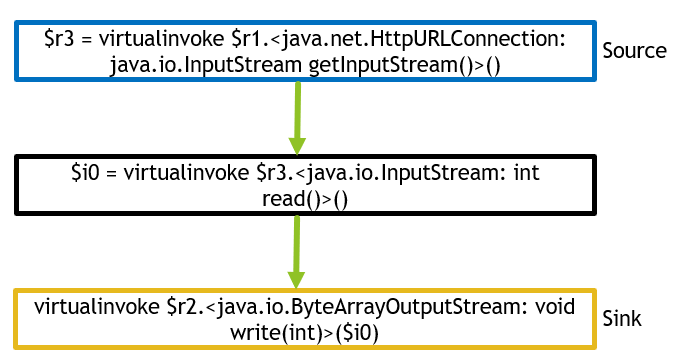
\includegraphics[width=5cm]{images/pathbenign.png} }}%
    \qquad
    \subfloat[\centering Path source/sink from malicious app]{{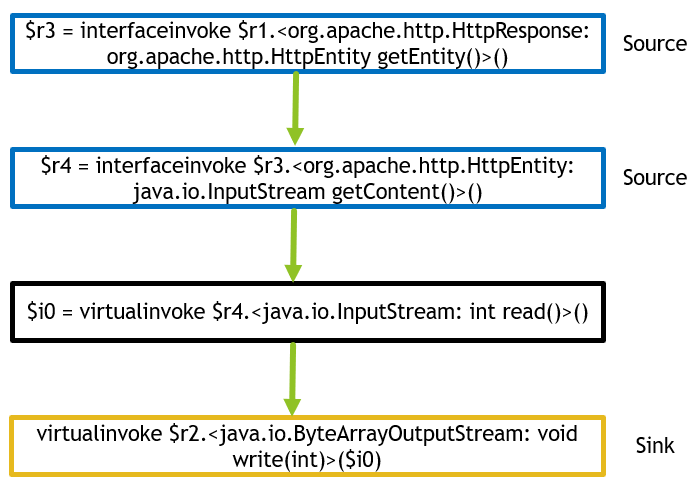
\includegraphics[width=5cm]{images/pathmalicious.png} }}%
    \caption{Pairs source/sink different (B/M)}%
    \label{fig:sourcesink}%
\end{figure}

\subsection{Discussion}\label{sec:discussion}

First we find that static analysis summaries had impact in the \blls. It was responsible for improving the results of the tools, between $16.44\%$ and $51.79\%$, discarding our Joker tool, answering our first research question (RQ1). Second, Table \ref{tab:fs} also summarizes our findings addressing the second research question (RQ2). We realized that disregarding the static analysis algorithms, and discarding Joker tool, among the tools analyzed in your study, Humanoid had the biggest performance drop, obtaining an effective performance of $28.12\%$, 27 malicious apps, among 96. The least affected was DroidBot, proving be the tool with better effective performance, in terms of the number of detected malware, obtaining an effective performance of $63.54\%$, 61 malicious apps, among 96 . Finally, we answered our last research question (RQ3) when we leverage sandboxes, complementing the dynamic analysis provided by test generation tool with tainted analysis algorithms. Our experiment highlight that $69.79\%$-$82.29\%$ of malware in dataset can be now uncovered by the complement of tainted analysis algorithms, evidencing that 
sandboxes can be further boosted when coupled with new static analysis techniques. We found that the number of identified malicious apps detected is increased for all cases, achieving at the best case, $82.29\%$ with DroidBot, a better performance than all five tools explored at \blls, even when they constructed a sandbox by combining all test generation tools at theirs work $75.49\%$. Table \ref{tab:tanted} display the increase of all tools explored at our research.

\begin{table}[ht]
\centering
\begin{tabular}{lccc}\toprule
 Test Generation & FlowDroid & Total & \%\\
 Tool & Increase  &  & \\ \midrule
 DroidBot & 6 & 79 & 82.29\\
 Monkey & 7 &  78 & 81.25 \\
 DroidMate & 7 & 75 & 78.12  \\
 Humanoid & 16 & 72 & 75.00 \\
 Joker & 25 & 67 & 69.79  \\\midrule
 
\end{tabular} 
\caption{Malwares detected in 96 pair (B/M) increased by Tainted analysis Algorithms}
\label{tab:tanted}
\end{table}


%%here we also have to write about the intersection between droidfax and tainted analysis now, and about what 1 reveled and other dont, and otherwise. 


%Here we can write about MOTIVATION EXAMPLES.
